\documentclass{article}
\usepackage[english]{babel}
\usepackage[utf8]{inputenc}
\usepackage{graphicx}
\usepackage{hyperref}
\graphicspath{ {graphics/} }

\title{CONTOUR BASED OPTICAL BRAILLE RECOGNITION FOR SINGLE SIDED ENGLISH BRAILLE TEXT}
\author{Divya Antony J.R.}
\date{March 2020}
\begin{document}
\maketitle

\section{Introduction}

\textbf{Optical Braille Recognition(OBR)} is the process or task of recognizing braille text from a simple image.
It is analogous to \textbf{Optical Character Recognition(OCR)}. For this problem we propose simple image processing 
instead of using complex structures like \emph{Artificial Neural Networks}. Some studies have used ANNs but we see
this unnecessary since single sided english braille is not something like handwritten digits which is very distinct,
It has some deformities due to wear and tear but braille characters most probably will not be handwritten 
and it also has a standard format to follow.

Thus we use shopisticated image processing and contours to decode the braille text. We see \textbf{OpenCV} is the best 
fit for implementing the proposed idea.

\section{Anatomy of Braille Text}

\begin{figure}[!htb]
\caption{The structure of a single braille character}
\centering
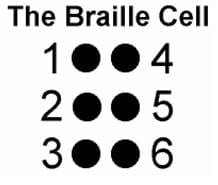
\includegraphics[scale=0.3]{braillecell}
\end{figure}



Braille is a tactile writing system used by people who are visually impaired. It is traditionally written with embossed paper.
These characters have \textbf{rectangular blocks called cells that have tiny bumps called raised dots}. The number and arrangement of these dots distinguish one character from another.

Since we are only looking at \textbf{English Braille}, the braille characters are very predictable. A single braille character can be 
contained in a \textbf{3x2 Matrix}, (i.e) A single braille character in English braille text is a grid of 3 rows and 2 columns.
This gives an opertunity to make the segmentation and processing optimal.

\emph{It is also worth to note that in our problem of recognizing English braille text, the first column of the braille in a
single braille character will have atleast one dot present. This makes the segmenting of the braille character much more
accurate}


\textbf{Thus a braille text contains a collection of braille cells as shown in figure 1 to form the entire text.}

\section{Preprocessing of the Braille Text Image}

First we do various image morphing techniques to reduce noise and increase sharpness of the dots in the 
braille text, We do this by the following steps,

\begin{enumerate}
  \item Conversion of \textbf{BGR/RGB scale to Gray scale}.
  \item Apply segmentation using \textbf{Binary Thresholding and OTSU Thresholding}.
  \item Remove Noise using \textbf{Blurring}
  \item Repeat the above process for \textbf{3 iterations}.
  \item Convert the result of the final thresholding to \textbf{binary image}.
\end{enumerate}

Now with the final binary image we find contours.

\subsection{Conversion to Gray scale}

\begin{figure}[!htb]
\caption{A image of Braille Text converted from RGB to Gray}
\centering
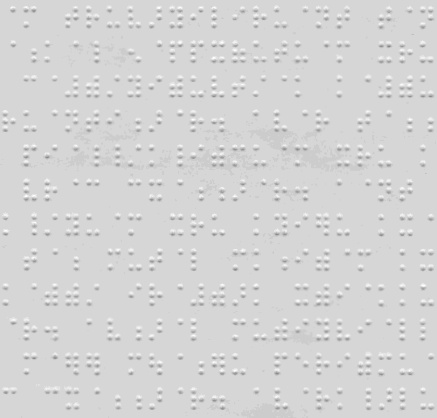
\includegraphics[scale=0.4]{gray}
\end{figure}



Using the following equation we convert the \textbf{RGB/BGR} to Gray channel.

\begin{equation}
	Y = (0.299*R) + (0.587*G) + (0.114*B)
\end{equation}

Here \textbf{Y} is the Gray channel which can be used to construct the Gray scale image.

\subsection{Segmentation using Binary Thresholding and OTSU Thresholding}

\begin{figure}[!htb]
\caption{Binary Thresholding of Braille Text}
\centering
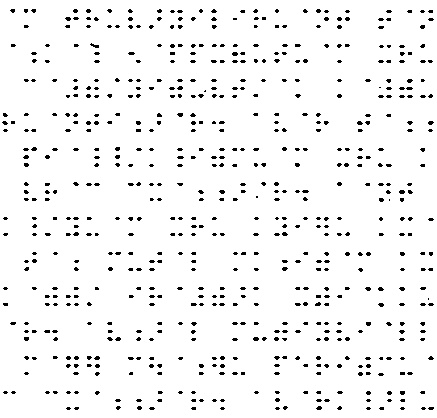
\includegraphics[scale=0.4]{binthresh}
\end{figure}


Thresholding is the \textbf{simplest form of segmentation}. Segmentation is the process in
which different regions of a image is identified. By identifying different regions, we 
can effectively find \textbf{the impressed dots in the image by segmenting it from the background}.

In our proposed solution we use a combination of \emph{Binary Thresholding} and \emph{OTSU Thresholding (invented by Nobuyuki Otsu)}.

\begin{equation}
Destination_{(x,y)} = \left\{
  \begin{array}{ll}
	  maxval & : Source(x,y) > T(x,y)\\
	  0 & : Otherwise
  \end{array}
\right.
\end{equation}

Where \textbf{T(x,y)} is the threshold of the pixel at x,y with respect to 2d cartesian plane.

Equation \textbf{(2)} is used for binary thresholding.

\[ \\ \]

The Otsu's algorithm tries to find a threshold value (t) which minimizes the \textbf{weighted within-class variance} given by the relation in equation \textbf{(3)} below,

\begin{equation}
\sigma_w^2(t) = q_1(t)\sigma_1^2(t)+q_2(t)\sigma_2^2(t)
\end{equation}

Where,

\[
q_1(t) = \sum_{i=1}^{t} P(i) \quad \& \quad q_2(t) = \sum_{i=t+1}^{I} P(i)
\]

\[
\mu_1(t) = \sum_{i=1}^{t} \frac{iP(i)}{q_1(t)} \quad \& \quad \mu_2(t) = \sum_{i=t+1}^{I} \frac{iP(i)}{q_2(t)}
\]


\[\sigma_1^2(t) = \sum_{i=1}^{t} [i-\mu_1(t)]^2 \frac{P(i)}{q_1(t)} \quad \& \quad \sigma_2^2(t) = \sum_{i=t+1}^{I} [i-\mu_2(t)]^2 \frac{P(i)}{q_2(t)}
\]

\subsection{Removing Noise}

\begin{figure}[!htb]
\caption{Gaussian blur applied to the Braille Text Gray Scale image}
\centering
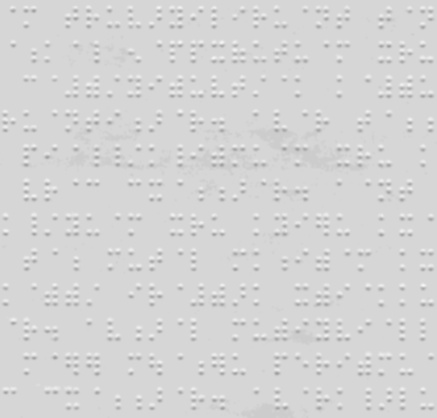
\includegraphics[scale=0.4]{gaussian}
\end{figure}

Using \textbf{Gaussian Blurring and Median Blurring} we reduce noise in the captured image as much as possible.

\subsection{Conversion to Binary Image}

Finally after all the processing, the final thresholded image is now converted to a binary image. (i.e) The image now has only two possible values for a single pixel.

\textbf{A high value represents a white pixel and a low value represents a black pixel}

\section{Contours}

\begin{figure}[!htb]
\caption{Contours drawn on the original image}
\centering
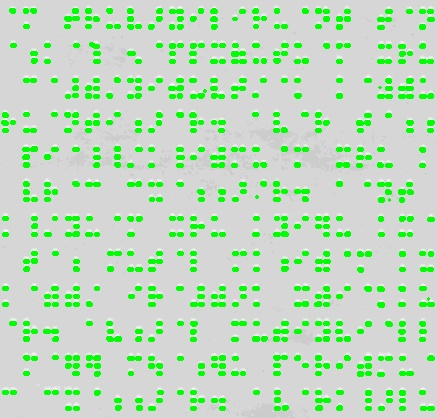
\includegraphics[scale=0.4]{contours}
\end{figure}


Contours are simple curve joining all the continuous points (along the boundary), having same color or intensity. The contours are useful tool for shape analysis and object detection and recognition. Contours can be extracted from the binary image which was obtained from the preprocessing step.

We find contours by a method proposed by \textbf{Satoshi Suzuki et el}. This method is already implemented in \textbf{OpenCV} so we need not define the entire algorithm as it exceeds the scope of this study.

Once we find the contours we do the \textbf{Braille Character Segmentation}.


\section{Braille Character Segmentation}


Segmentation is very simply built and unique to our study. The main feature about this segmentation is that this research can be further improved with Artificial Neural Networks if desired as this segmentation allows us to separate individual braille character with all the pixel data required for Convolutional Neural Networks.

The Segmentation process is as follows,


\begin{enumerate}
  \item Calculate the \textbf{Mean Radius and Diameter} of each dots in each Braille Character using the Contours.
  \item Using the Radius and Diameter, Find the \textbf{Center Point} of all dots in each Braille Characters.
  \item Find the smallest \textbf{Center Point} of all dots in each Braille Characters in both X and Y Axis.
  \item With the X and Y points find all possible Braille Characters as \textbf{3x2} matrix.
  \item Get each Braille Character bounding Rectangle Coordinates.
  \item With the bounding Rectangle Coordinates, Each Braille Character can be Segmented.
\end{enumerate}

With each Braille Character segmented as separate images we can do simple image processing to convert the image to a \textbf{3x2} matrix, this matrix can be converted to \textbf{vector with single dimension}. Each combination of such vectors will represent a character in English, Thus a sentence can be constructed.


\begin{figure}[!htb]
\caption{Braille Characters Bounded by a Bounding Rectangle}
\centering
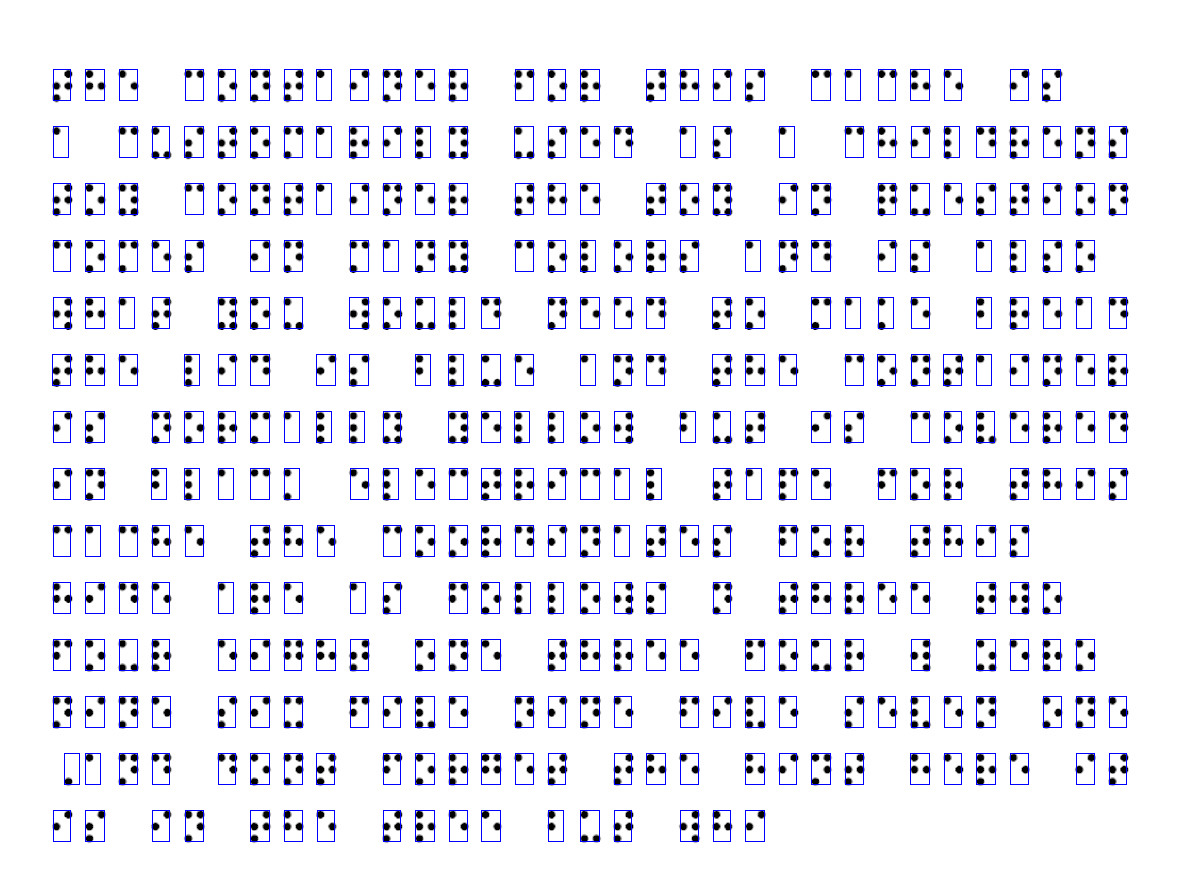
\includegraphics[scale=0.2]{rectangle}
\end{figure}

\section{Future Works}

In future we propose to use Convolution Neural Network to classify each Braille Image for better accuracy and classification instead of using a Combination Hash Table as used in our Study.


\section{Conclusion}

Our study was able to do the segmentation and Braille Recognition in real time and at a state-of-the-art speed compared to any Artificial Neural Network based Segmentation methods. This Braille Recognition can be done in low powered devices also since we do not use complex system like Convolutional Neural Network. The accuracy is on par with any Aritficial Neural Network based Braille Recognition to the best of our knowledge with \textbf{98.457\%}.

We believe that this study can be deployed in Mobile Systems with ease compared to Artificial Neural Network based Braille Recognition.



\section{Miscellaneous}

The source code of this entire study can be found at \href{https://github.com/antony-jr/OpticalBrailleRecognition}{github} which is licensed under \textbf{The BSD 3-clause "New" or "Revised" License.}



A application to demonstrate this study is hosted at \href{https://opticalbraillerecognition-demo.herokuapp.com/}{heroku}.

\end{document}
